\subsection{求解二次规划问题的积极集法}
\label{subsec:7.2.2}
% finished

对于一般的带不等式约束的二次规划问题~\eqref{eq:quadratic-programming-1}, 有一系列的实用算法来求解这些问题. 经典的积极集法~(active-set methods) 自从~20 世纪~70 年代起被广泛应用于求解二次规划问题. 积极集法适用于求解中小规模~(成百上千个变量) 的凸和非凸的二次规划问题. 梯度投影法~(gradient-projection methods) 是属于积极集法的一种特殊的算法, 是经典积极集法的推广, 能够非常高效地求解简单约束的二次规划问题, 例如对每个变量的约束都是区间约束的二次规划问题~($a_i \leqslant x_i \leqslant b_i,$ 称这样的问题为~BoxQP). 还有一类方法是内点法~(interior-point methods), 广泛应用于求解二次规划问题的时间比经典积极集法稍晚, 大概始于~20 世纪~90 年代. 内点法适用于求解大规模的凸二次规划问题. 本节主要介绍如何利用积极集法将等式约束问题的求解方法推广以求解带不等式约束的二次规划问题. 为描述简单, 假设原问题是凸二次规划问题.

回顾一下, 对于二次规划问题~\eqref{eq:quadratic-programming-1}, 积极集~$\mathcal{A}(x)$ 的定义为
\begin{equation}
\label{eq:qp-active-set}
\mathcal{A} = \mathcal{A}({x}) = \left\{ i : ~ {a}_i^T {x} = b_i, ~ i \in \mathcal{E} \cup \mathcal{I} \right\},
\end{equation}
即在点~${x}$ 处, 等式成立的约束条件的指标~(index) 组成的集合. 
将一般的二次规划的~KKT 条件~\eqref{eq:quadratic-programming-kkt} 根据积极集~$\mathcal{A}({x}^*)$ 改写一下, 即有
\begin{equation}
\label{eq:qp-active-set-kkt}
\begin{aligned}
& G {x}^* + d + \sum\limits_{i \in \mathcal{A}({x}^*)} \lambda_i^* {a}_i = {0}, \\
& {a}_i {x}^* = b_i, ~~ \forall i \in \mathcal{A}({x}^*), \\
& {a}_i {x}^* \leqslant b_i, ~~ \forall i \in \mathcal{I} \setminus \mathcal{A}({x}^*), \\
& \lambda_i^* \geqslant 0, ~~ \forall i \in \mathcal{I} \cap \mathcal{A}({x}^*).
\end{aligned}
\end{equation}
不难发现, ${x}^*$ 也是下面等式问题的~KKT 点
\begin{equation}
\label{eq:qp-active-set-1}
\begin{array}{cl}
\min & \frac{1}{2} {x}^T G {x} + {d}^T {x}, \\
{\rm s.t.} & {a}_i^T {x} = b_i, ~ i \in \mathcal{A}({x}^*).
\end{array}
\end{equation}
这说明, 求解含不等式约束的二次规划问题几乎~(注意~KKT 条件~\eqref{eq:qp-active-set-kkt} 中的最后两个条件) 等价于求解一个等式约束的二次规划问题, 如果事先知道~$\mathcal{A}({x}^*).$ 但通常这是不可能的, 因此不能通过求解等式问题~\eqref{eq:qp-active-set-1} 来求解原二次规
划问题~\eqref{eq:quadratic-programming-1}.

在积极集法中, 依据以上的观察, 将积极集~$\mathcal{A}$ 确定的约束看作等式约束, 而暂时忽略其余约束条件, 并通过某种迭代的方式不断修正调整这个集合, 直到识别出原问题~\eqref{eq:quadratic-programming-1} 的解处的正确的积极约束. 更具体来说, 在第~$k$ 次迭代, 从可行点~${x}^{(k)}$ 出发, 
积极集为~$\mathcal{A} = \mathcal{A}({x}^{(k)}).$ 在这一步迭代中, 
求解等式问题~\eqref{eq:qp-active-set-1}. 更方便的做法是将原点平移到~${x}^{(k)},$ 令~${s} = {x} - {x}^{(k)},$ 求解问题
\begin{equation}
\label{eq:qp-active-set-2}
\begin{array}{cl}
\min & \frac{1}{2} {s}^T G {s} + \left( {g}^{(k)} \right)^T {s}, \\
{\rm s.t.} & {a}_i^T {s} = 0, ~ i \in \mathcal{A},
\end{array}
\end{equation}
其中~${g}^{(k)} = \nabla q({x}^{(k)}) = G {x}^{(k)} + {d}$ 是原二次
规划问题~\eqref{eq:quadratic-programming-1} 的目标函数~$q({x})$ 在点~${x}^{(k)}$ 处的梯度向量.  这个问题是一个等式约束的二次规划问题, 可以用上一小节~\S\ref{subsec:7.2.1} 中介绍的等式约束二次规划问题的求解方法进行求解. 记问题~\eqref{eq:qp-active-set-2} 的解为~${s}^{(k)},$ 需要对各种可能的情况进行分类讨论.

如果~${s}^{(k)} = {0},$ 即~${x}^{(k)}$ 是当前等式约束问题~\eqref{eq:qp-active-set-1} 的解, 那么可以根据式~\eqref{eq:general-elim-lagrange} 计算积极约束的拉格朗日乘子, 记为~${\lambda}^{(k)},$  即有
\begin{equation}
\label{eq:qp-active-set-lambda}
{g}^{(k)} + \sum\limits_{i \in \mathcal{A}} \lambda_i^{(k)} \alpha_i = 0.
\end{equation}
此时, 除对偶可行性条件~$\lambda_i \geqslant 0, ~ i \in \mathcal{I}$ 以外, 其余~KKT 
条件~\eqref{eq:qp-active-set-kkt} 均满足. 当与原问题不等式约束对应的拉格朗日乘子均非负, 即
\begin{equation*}
\lambda_i^{(k)} \geqslant 0, ~ \forall i \in \mathcal{I} \cap \mathcal{A},
\end{equation*}
则~$x^{(k)}$ 是原问题的~KKT 点, 迭代结束, 求解完毕. 若不然, 则设
\begin{equation}
\label{eq:qp-active-set-inactive-index}
q = \argmin_{i \in \mathcal{I} \cap \mathcal{A}} \lambda_i^{(k)},
\end{equation}
有~$\lambda_q^{(k)} < 0.$ 令~$\mathcal{A} = \mathcal{A} \setminus \{ q \},$ 
代入问题~\eqref{eq:qp-active-set-2}, 并求解此新的子问题.

如果~${s}^{(k)} \neq {0},$ 即~${x}^{(k)}$ 不是当前等式约束问题~\eqref{eq:qp-active-set-1} 的解, 那么进一步检验试探点
\begin{equation}
\label{eq:qp-active-set-test-point}
\bar{{x}}^{(k)} = {x}^{(k)} + {s}^{(k)}
\end{equation}
是否满足其他不在积极集~$\mathcal{A}$ 中的不等式约束条件. 如果都满足的话, 令
\begin{equation}
\label{eq:qp-active-set-next-step-1}
{x}^{(k+1)} = \bar{{x}}^{(k)} = {x}^{(k)} + {s}^{(k)},
\end{equation}
积极集保持不变, 进入下一步迭代搜索. 如果不然, 即存在指标~$i \not\in \mathcal{A},$ 使得
\begin{equation*}
{a}_i^T {x}^{(k)} - {b} + {s}^{(k)} > 0,
\end{equation*}
此时试探点~$\bar{{x}}^{(k)}$ 不是原问题的可行点, 需要将其投影到原问题的可行域. 
沿着方向~${p}^{(k)} = {s}^{(k)}$ 进行线搜索, 选一个小于~$1$ 但尽可能大的步长
\begin{equation}
\label{eq:qp-active-set-step-len-1}
\begin{aligned}
\bar{\alpha}_k & = \max \left\{ \alpha : ~ \alpha > 0, ~ {a}_i^T {x}^{(k)} - b_i + \alpha {a}_i^T {p}^{(k)} \leqslant 0, ~ {a}_i^T {p}^{(k)} > 0, ~ \forall i \not\in \mathcal{A} \right\}, \\
& = \min_{\substack{i: i \not\in \mathcal{A} \\ {a}_i^T {p}^{(k)} > 0}} \frac{b_i - {a}_i^T {x}^{(k)}}{{a}_i^T {p}^{(k)}}.
\end{aligned}
\end{equation}
注意~$\bar{\alpha}_k$ 是严格小于~$1$ 的, 因为此时的试探点~${x}^{(k)} + {s}^{(k)}$ 不可行. 取指标~$j$ 使得第~$j$ 个约束取得上式中~$\frac{b_i - {a}_i^T {x}^{(k)}}{{a}_i^T {p}^{(k)}}$ 的最大值, 即
\begin{equation}
\label{eq:qp-active-set-step-len-2}
\bar{\alpha}_k = \frac{b_j - {a}_j^T {x}^{(k)}}{{a}_j^T {p}^{(k)}}, ~~ j = \argmin_{\substack{i: i \not\in \mathcal{A} \\ {a}_i^T {p}^{(k)} > 0}} \frac{b_i - {a}_i^T {x}^{(k)}}{{a}_i^T {p}^{(k)}},
\end{equation}
并称指标~$j$ 对应的约束为阻滞~(blocking) 约束. 取
\begin{equation}
\label{eq:qp-active-set-next-step-2}
{x}^{(k+1)} = {x}^{(k)} + \bar{\alpha}_k {s}^{(k)}, ~~ \mathcal{A} \gets \mathcal{A} \cup \{ j \}.
\end{equation}
这里把指标~$j$ 添加到了积极集, 是因为对于~${x}^{(k+1)},$ 指标~$j$ 对应的约束条件等式成立, 非积极约束~$j$ 变成积极的. 迭代格式~\eqref{eq:qp-active-set-next-step-1}
与~\eqref{eq:qp-active-set-next-step-2} 可以统一表述为: 以等式问题~\eqref{eq:qp-active-set-2} 
的解~${s}^{(k)}$ 为搜索方向~${p}^{(k)},$ 以
\begin{equation}
\label{eq:qp-active-set-step-len-uniform}
\alpha_k = \min (1, \bar{\alpha}_k)
\end{equation}
为迭代步长, 得下一步的迭代点
\begin{equation}
\label{eq:qp-active-set-next-step-uniform}
{x}^{(k+1)} = {x}^{(k)} + \alpha_k {p}^{(k)},
\end{equation}
同时根据是否有阻滞约束确定是否更新积极集: 若~$\alpha_k < 1,$ 有约束阻滞~$j,$ 则将~$j$ 添加到积
极集~$\mathcal{A}.$

至此, 可以以伪代码的形式, 将经典的积极集法表示为算法~\ref{algo:active-set}.
\begin{algorithm}[htbp]
\caption{求解带不等式约束的二次规划
问题~\eqref{eq:quadratic-programming-1} 的积极集法}\label{algo:active-set}
\begin{algorithmic}[1]
\STATE 给定~$n$ 阶对称阵~$G,$ 列满秩的~$n \times m$ 的矩阵~$A,$ ${d} \in \mathbb{R}^n, {b} \in \mathbb{R}^m,$ 等式约束的数量~$m_1$. 随机选取一个可行点~${x}^{(0)},$ 确定相应
的积极集~$\mathcal{A},$ $k \gets 0.$

\STATE 求等式约束二次规划问题~\eqref{eq:qp-active-set-2} 解~${s}^{(k)}$.

\STATE 若~${s}^{(k)} = 0$, 由~\eqref{eq:qp-active-set-lambda} 式计算拉格朗
日乘子~${\lambda}^{(k)}$, 计算指标~$q \gets \argmin\limits_{i \in \mathcal{I} \cap \mathcal{A}} \lambda_i^{(k)}$.

\STATE 若~$\lambda^{(k)}_q \geqslant 0$, ${x}^* \gets {x}^{(k)}$, 算法终止, 返回~${x}^*$. 否则, ${x}^{(k+1)} \gets {x}^{(k)}$, 将指标~$q$ 从积极集~$\mathcal{A}$ 中移除: $\mathcal{A} \gets \mathcal{A} \setminus \{ j \}$.

\STATE 取线搜索方向~${p}^{(k)} \gets {s}^{(k)}$, 由式~\eqref{eq:qp-active-set-step-len-2} 
计算~$\bar{\alpha}_k$ 以及相应的约束条件的指标$j$, 取步长~$\alpha_k \gets \min (1, \bar{\alpha}_k)$, 令~${x}^{(k+1)} \gets {x}^{(k)} + \alpha_k {p}^{(k)}$.


\STATE 若~$\alpha_k < 1$, 将阻滞约束条件的指标~$j$ 添加到积极集~$\mathcal{A}$ 中: $\mathcal{A} \gets \mathcal{A} \cup \{ j \}$. 

\STATE 令~$k=k+1$, 转步~2.
\end{algorithmic}
\end{algorithm}

\begin{exam}\label{eg:qp-active-set-algo}
下面举例说明用积极集法求解含不等式约束的二次规划问题的步骤. 考虑如下的二次规划问题
\begin{equation*}
\begin{array}{cl}
\min & q({x}) = (x_1 - 1)^2 + (x_2 - 2.5)^2, \\
{\rm s.t.} & -x_1 + 2x_2 - 2 \leqslant 0, \\
& x_1 + 2x_2 - 6 \leqslant 0, \\
& x_1 - 2x_2 - 2 \leqslant 0, \\
& -x_1 \leqslant 0, \\
& -x_2 \leqslant 0,
\end{array}
\end{equation*}
用积极集法进行求解. 该问题的可行域可见图~\ref{fig:active-set-eg}, 由其中实线以及坐标轴围成的阴影区域构成.

% \begin{figure}[htpb]\label{fig:active-set-eg}
% \centering
% 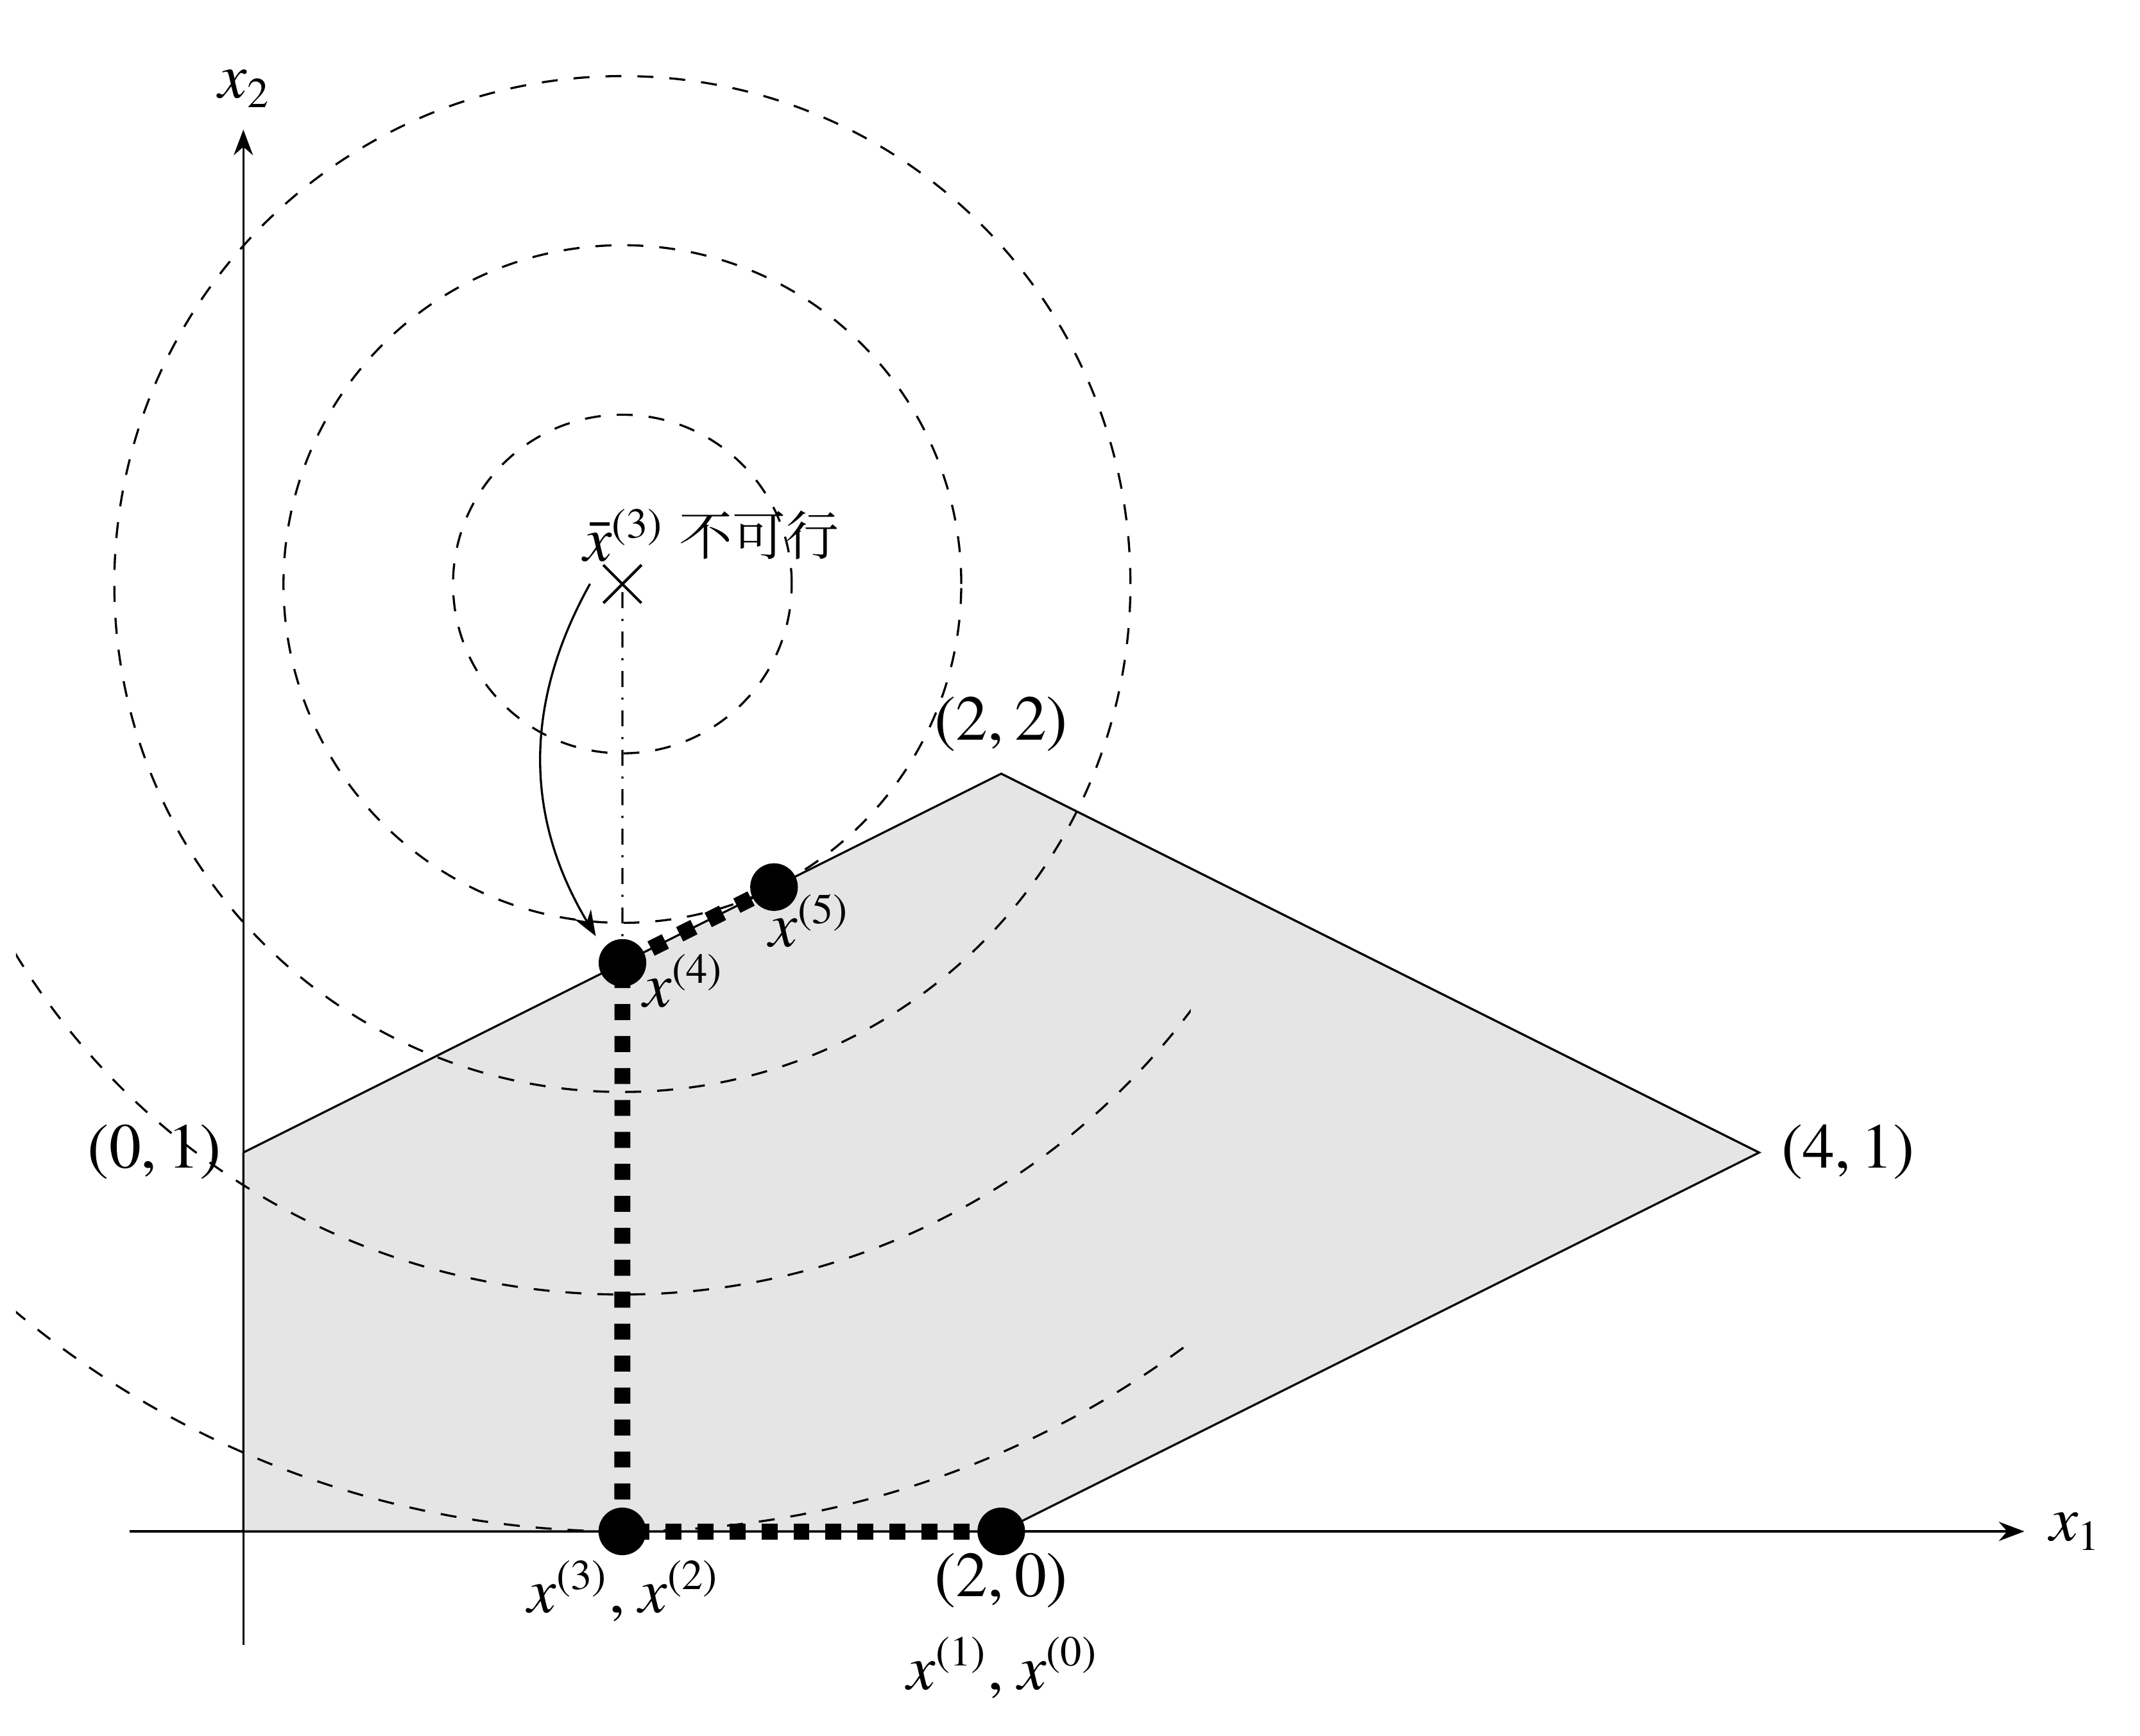
\includegraphics[width=0.75\textwidth]{fig-qp-active-set.png}
% \caption{积极集法求解例~\ref{eg:qp-active-set-algo} 的迭代示意图}
% \end{figure}

\begin{figure}[ht]
\centering
\larger[1]
\begin{tikzpicture}[scale=2.3, circle defined by/.style args={center #1 and point #2}{insert path={let \p1=($(#2)-(#1)$),\n1={veclen(\x1,\y1)} in (#1) circle[radius=\n1]}}]
% \draw[gray!30, thin, dashed] (-0.5, -0.5) grid (4.6, 3.9);
\coordinate (C) at (1, 2.5);
% coordinate axes
\draw[-{Stealth}] (-0.5, 0)--(4.7, 0) node [right] {$x_1$};
\draw[-{Stealth}] (0, -0.5)--(0, 3.7) node [above] {$x_2$};
% feasible region
\draw[fill=gray!20] (0, 1) node (p1) [left] {$(0, 1)$} -- (2, 2) node (p2) [above] {$(2, 2)$} -- (4, 1) node (p3) [right] {$(4, 1)$} -- (2, 0) node (p4) [below] {$(2, 0)$} -- (0, 0);
% iterations of the active-set algorithm
\node[below = -0.1 of p4] (x01) {$\V{x}^{(0)}, \V{x}^{(1)}$};
\draw[dashed, line width=3] (2, 0) -- (1, 0) node (x23) [below] {$\V{x}^{(2)}, \V{x}^{(3)}$};
\path[name path = line1] (0, 1) -- (2, 2);
\path[name path = vertical1] (1, 0) -- (1, 4);
\draw[dashed, line width=3, name intersections = {of = line1 and vertical1, by = {x4}}]  (1, 0) -- (x4);
\node[above = -0.1 of x4] {$\V{x}^{(4)}$};
\coordinate (c1) at (0, 1);
\coordinate (c2) at (2, 2);
\coordinate (x5) at ($(c1)!(C)!(c2)$);
\draw[dashed, line width=3] (x4) -- (x5);
\node[above = -0.1 of x5] {$\V{x}^{(5)}$};
% contour: circles
\begin{scope}
% \clip (-.6, -.3) rectangle (3, 3.2);
\draw[dashed, circle defined by=center C and point x5];
\coordinate (midx5) at ($(C)!0.5!(x5)$);
\draw[dashed, circle defined by=center C and point midx5];
\coordinate (p6) at ($(C)!1.5!(x5)$);
\draw[dashed, circle defined by=center C and point p6];
\end{scope}
% contour: arcs
\begin{scope}
\clip (-.6, -.3) rectangle (2.5, 1.9);
\coordinate (p7) at (1, 0);
\draw[dashed, circle defined by=center C and point p7];
\coordinate (p8) at ($(C)!0.75!(p7)$);
\draw[dashed, circle defined by=center C and point p8];
\end{scope}
\end{tikzpicture}
\caption{积极集法求解例\ref{eg:qp-active-set-algo}的迭代示意图}
\label{fig:active-set-eg}
\end{figure}


选取初始点~${x}^{(0)} = (2, 0)^T,$ 用~$1$ 至~$5$ 依次作为约束条件的指标. 在初始点~${x}^{(0)}$ 处, 约束~$3$ 和~$5$ 满足等式关系, 是积极约束, 所以初始积极集~$\mathcal{A} = \{ 3, 5 \}.$ 当前需要求解的等式问题~\eqref{eq:qp-active-set-1} 为
\begin{equation*}
\begin{array}{cl}
\min & q({x}) = (x_1 - 1)^2 + (x_2 - 2.5)^2, \\
{\rm s.t.} & x_1 - 2x_2 - 2 = 0, \\
& x_2 = 0,
\end{array}
\end{equation*}
或者经过平移的问题~\eqref{eq:qp-active-set-2}
\begin{equation*}
\begin{array}{cl}
\min & q({s}) = (s_1 + 1)^2 + (s_2 - 2.5)^2, \\
{\rm s.t.} & s_1 - 2s_2 = 0, \\
& s_2 = 0.
\end{array}
\end{equation*}
很容易看到~${x}^{(0)}$ $($即~${s}^{(0)} = {0}$$)$ 是该问题的解. 
由式~\eqref{eq:qp-active-set-lambda} 求解积极约束的拉格朗日乘子, 即求解方程组
\begin{equation*}
\begin{bmatrix} 1 \\ -2 \end{bmatrix} \lambda_3^{(0)} + \begin{bmatrix} 0 \\ -1 \end{bmatrix} \lambda_5^{(0)} = \begin{bmatrix} -2 \\ 5 \end{bmatrix},
\end{equation*}
得~$\lambda_3^{(0)} = -2, \lambda_5^{(0)} = -1.$ 指标~$q = \argmin\limits_{i \in \{ 3, 5 \}} \lambda_i^{(0)} = 3.$ 由于~$\lambda_q^{(0)} = \lambda_3^{(0)} = -2 < 0,$ 因此置~${x}^{(1)} = {x}^{(0)},$ 同时将指标~$q = 3$ 从积极集中删去, 进入下一步迭代. 接下来需要求解等式问题
\begin{equation*}
\begin{array}{cl}
\min & q({s}) = (s_1 + 1)^2 + (s_2 - 2.5)^2, \\
{\rm s.t.} & s_2 = 0.
\end{array}
\end{equation*}
容易解得~${s}^{(1)} = (-1, 0)^T.$ 此时, 试探点~${x}^{(1)} + {s}^{(1)} = (1, 0)^T$ 是可行点,  置~${x}^{(2)} = {x}^{(1)} + {s}^{(1)} = (1, 0)^T,$ 同时积极集~$\mathcal{A} = \{ 5 \}$ 保持不变, 进入下一步迭代. 容易验证~${x}^{(2)}$ 是这一步要解的等式问题的可行解, 进而可计算得相应的积极约束的拉格朗日乘子~$\lambda_5^{(2)} = -5.$ 此时, 约束~$5$ 变成非积极的, 积极集~$\mathcal{A} = \emptyset$ 变为空集. 置~${x}^{(3)} = {x}^{(2)} = (1, 0)^T$ 进入下一步迭代. 再次求解当前的等式约束问题~$($实际上已成为无约束问题$)$
\begin{equation*}
\min ~~ q({s}) = s_1^2 + (s_2 - 2.5)^2,
\end{equation*}
得解~${s}^{(3)} = (0, 2.5)^T.$ 试探点~${x}^{(3)} + {s}^{(3)} = (1, 2.5)^T$ 不是可行点, 
因此需要以~${p}^{(3)} = {s}^{(3)}$ 为方向进行线搜索~${x}^{(3)} + \alpha_3 {p}^{(3)},$ 
并由式~\eqref{eq:qp-active-set-step-len-2} 以及式~\eqref{eq:qp-active-set-step-len-uniform} 算得最优步长~$\alpha_3 = 0.6,$ 以及相应阻滞约束的指标~$j = 1.$ 置~${x}^{(4)} = {x}^{(3)} + \alpha_3 {p}^{(3)} = (1, 1.5)^T,$ 并将阻滞约束的指标~$j = 1$ 添加到积极集得~$\mathcal{A} = \{ 1 \},$ 进入下一步迭代. 再次求解当前的等式问题, 得~${s}^{(4)} = (0.4, 0.2)^T.$ 相应的试探点~${x}^{(4)} + {s}^{(4)} = (1.4, 1.7)^T$ 可行, 于是得新的迭代点~${x}^{(5)} = (1.4, 1.7)^T.$ 由于~${x}^{(5)}$ 是当前等式问题的可行点, 且解得积极约束的拉格朗日乘子~$\lambda_1^{(5)} = 0.8 > 0,$ 算法终止条件达成,  得原问题的最优解
\begin{equation*}
{x}^* = {x}^{(5)} = (1.4, 1.7)^T.
\end{equation*}
将每一步的数值结果总结在表~\ref{tab:active-set-eg} 中. 表中的``$\backslash$''表示当前迭代步不需要计算相应的量.
\begin{table}[H]
    \caption{积极集法求解例~\ref{eg:qp-active-set-algo} 数值结果}
    \label{tab:active-set-eg}
    \centering
    \begin{tabular}{cccccccccc}
    \hline
    $k$ & ${x}^{(k)}$ & $\mathcal{A}$ & ${s}^{(k)}$ & $\bar{{x}}^{(k)}$可行 & ${\lambda}^{(k)}$ & $q$ & $\alpha_k$ & $j$ & $q({x}^{(k)})$ \\
    \hline
    \multirow{2}{*}{$0$} & \multirow{2}{*}{$(2, 0)^T$} & \multirow{2}{*}{$\{ 3, 5 \}$} & \multirow{2}{*}{$(0, 0)^T$} & \multirow{2}{*}{$\checkmark$} & $\lambda_3^{(0)} = -2$ & \multirow{2}{*}{$3$} & \multirow{2}{*}{$0$} & \multirow{2}{*}{$\backslash$} & \multirow{2}{*}{$7.25$} \\
    & & & & & $\lambda_5^{(0)} = -1$ & & & \\
    $1$ & $(2, 0)^T$ & $\{ 5 \}$ & $(-1, 0)^T$ & $\checkmark$ & $\backslash$ & $\backslash$ & $1$ & $\backslash$ & $7.25$ \\
    $2$ & $(1, 0)^T$ & $\{ 5 \}$ & $(0, 0)^T$ & $\checkmark$ & $\lambda_5^{(2)} = -5$ & $5$ & $0$ & $\backslash$ & $6.25$ \\
    $3$ & $(1, 0)^T$ & $\emptyset$ & $(0, 2.5)^T$ & $\times$ & $\backslash$ & $\backslash$ & $0.6$ & $1$ & $6.25$ \\
    $4$ & $(1, 1.5)^T$ & $\{ 1 \}$ & $(0.4, 0.2)^T$ & $\checkmark$ & $\backslash$ & $\backslash$ & $1$ & $\backslash$ & $1$ \\
    $5$ & $(1.4, 1.7)^T$ & $\{ 1 \}$ & $(0, 0)^T$ & $\checkmark$ & $\lambda_1^{(5)} = 0.8$ & $\backslash$ & $\backslash$ & $\backslash$ & $0.8$ \\
    \hline
    \end{tabular}
\end{table}
\end{exam}
